%\documentstyle[epsf,twocolumn]{jarticle}       %LaTeX2e仕様
%\documentclass[twocolumn]{jarticle}     %pLaTeX2e仕様(platex.exeの場合)
\documentclass[onecolumn]{ujarticle}   %pLaTeX2e仕様(uplatex.exeの場合)
%%%%%%%%%%%%%%%%%%%%%%%%%%%%%%%%%%%%%%%%%%%%%%%%%%%%%%%%%%%%%%
%%
%%  基本バージョン
%%
%%%%%%%%%%%%%%%%%%%%%%%%%%%%%%%%%%%%%%%%%%%%%%%%%%%%%%%%%%%%%%%%
\setlength{\topmargin}{-45pt}
%\setlength{\oddsidemargin}{0cm}
\setlength{\oddsidemargin}{-7.5mm}
%\setlength{\evensidemargin}{0cm}
\setlength{\textheight}{24.1cm}
%setlength{\textheight}{25cm}
\setlength{\textwidth}{17.4cm}
%\setlength{\textwidth}{172mm}
\setlength{\columnsep}{11mm}

%\kanjiskip=.07zw plus.5pt minus.5pt


% 【節が変わるごとに (1.1)(1.2) … (2.1)(2.2) と数式番号をつけるとき】
%\makeatletter
%\renewcommand{\theequation}{%
%\thesection.\arabic{equation}} %\@addtoreset{equation}{section}
%\makeatother

%\renewcommand{\arraystretch}{0.95} 行間の設定
%%%%%%%%%%%%%%%%%%%%%%%%%%%%%%%%%%%%%%%%%%%%%%%%%%%%%%%%
%\usepackage{graphicx}   %pLaTeX2e仕様(\documentstyle ->\documentclass)
\usepackage[dvipdfmx]{graphicx}
\usepackage{subcaption}
\usepackage{multirow}
\usepackage{amsmath}
\usepackage{url}
%%%%%%%%%%%%%%%%%%%%%%%%%%%%%%%%%%%%%%%%%%%%%%%%%%%%%%%%
\begin{document}

	%bibtex用の設定
	%\bibliographystyle{ujarticle}
	\noindent

	\hspace{1em}
	2020 年 4 月 24 日
	ゼミ資料
	\hfill
	M2 寺内 光

	\vspace{2mm}

	\hrule

	\begin{center}
		{\Large \bf 進捗報告}
	\end{center}


	\hrule
	\vspace{3mm}

	% ‚ここから 文章 Start!
	\section{今週やったこと}
	\begin{itemize}{
		\item{DEAPを使うためのリポジトリ環境整備}
		\item{強化学習を用いたデータオーギュメンテーションの論文調査}
	}\end{itemize}
	\subsection{DEAP を使うためのリポジトリ環境整備}
	Docker+Make+PyTorch(Catalyst)で DEAP 環境を整えた.
	PyTorch のデータセットを継承したミニ版の Cifer-10 と MNIST でクラス分類タスクの動作確認.
	レポは\url{https://github.com/1g-hub/DEAP_CLS}に置いています.


	\subsection{強化学習を用いた Data Augmentationの論文調査}
	森先生がチャンネルにあげてくれていた \cite{8953317} を読んだ.以下,要約.
	\subsubsection{モチベーション}
	データをかさ増しする研究は少なく,あるかさ増し手法が他のデータセットにうまく効くかは不明.
	よって,このかさ増し操作の選択を強化学習を用いて自動で行いたい.

	\subsubsection{問題設定}
	このかさ増し操作を離散探索問題として設定し 5 つのサブポリシーをもつポリシーを探索する.各サブポリシーは2つの順序ある処理を含み,それぞれに対して適用確率(10\%刻みの11段階)と操作の大きさ(10段階)を持つ.操作は 16 種(Shear X/Y, TranslateX/Y, Rotate, AutoContrast, Invert, Equalize, Solarize, Posterize, Contrast, Color, Brightness, Sharpness, Cutout, SamplePairing).AutoContrast, Equalize はヒストグラムの補正を行う操作.Solarize はしきい値のついた Invert処理.Posterize は減色(量子化)操作.Cutout(Random Erasing) \cite{DBLP:journals/corr/abs-1708-04552, DBLP:journals/corr/abs-1708-04896} は 2017 年の 8 月に公開された操作で,画像の一部に画像の画素の平均値でマスクをかける.SamplePairing \cite{DBLP:journals/corr/abs-1801-02929} は 2018 年の 9月 に公開された操作で,異なる 2 枚の画像を重ねてそれを学習データに追加する.単純にデータ数が累乗レベルで増える.ラベルはもとの画像の一方のラベルを与える.クラスが違う画像間のこんな操作をしてもよいのかというのが純粋な疑問点だったが,同じラベルのペアよりもすべての画像を用いたほうが精度が上がったらしい..原著読むと書いてあるのかも?

	また,各サブ方策の探索空間は $(16*10*11)^2$ 通りで方策の探索空間は $(16*10*11)^{10} = 2.9*10^{32}$通り.

  \subsubsection{探索手法}
	強化学習ベース.コントローラは RNN で,各探索における検証精度を受け取り,方策勾配法により更新.
	各ミニバッチ内の画像 1 枚 1 枚に対し,5 つのサブポリシーの内 1 つを適用(一様乱数から選択)して学習する.
	CIFER-10, SVHN, ImageNet, FGVC を小さくしたデータセットで探索後.大きなデータセットでテスト.
	テスト時は最適なポリシー 5 こを展開したサブポリシー 25 こからなる 1 つのポリシーを用いる.
	図 \ref{fig:AutoAugment} に探索の全体像を示す.
	\begin{figure}
		\begin{center}
		  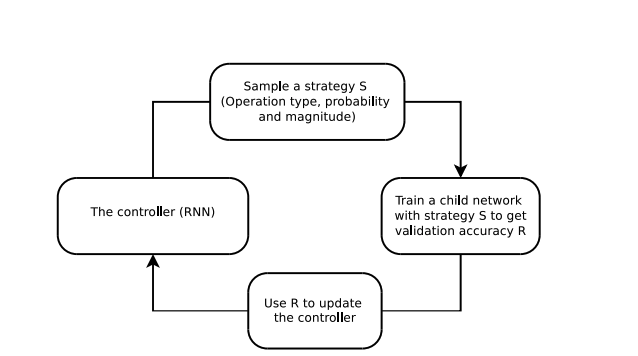
\includegraphics[width=13cm]{AutoAugment.png}
			\caption{AutoAugment 全体像}
			\label{fig:AutoAugment}
		\end{center}
	\end{figure}

	\subsubsection{結果}
	AutoAugment-direct(ミニデータで学習後,そのまま大きいデータセットに適用する) では CIFER-10, CIFER-100, SVHN, ImageNet データセットで SoTA を達成(追加データなし).各データセットに対し効果的な異なる方策が選択されていた.また,AutoAugment-transfer(ミニデータで学習後,別のデータセットに適用する)では多くのデータセットやモデルアーキテクチャ間での転移可能性を示した.しかし,転移に関してはデータ分布が近いものでないと効果が低いという考察もされている.
	また,操作が確率的なものであるため,child models(探索中のネットワーク)は 80 から 100 エポック(論文中は120エポック),full model(探索済みのモデル)はそれ以上に回す必要があると言及されている.

	\subsubsection{個人的な感想,GA 研究への応用}
	あまり目を向けられていない AutoML の Data Augmentation への適用研究はそれだけで見てて面白かった.論文中で探索方法次第ではより良くなる可能性がある,と示唆されており,強化学習(方策勾配法)での探索の部分に GA を適用することができそう.以下,論文より他の探索手法や GA への適用に関する言及があった部分を引用(ところどころで言及されている).

	\begin{quote}
		1. In our experiments, we use Reinforcement Learning as the search algorithm, but we believe the results can be further improved if better algorithms are used.

		2. We choose to train the controller using PPO out of convenience, although prior work had shown that other methods (e.g. augmented random search and evolutionary strategies) can perform as well or even slightly better.

		3. The above search algorithm is one of many possible search algorithms we can use to find the best policies. It might be possible to use a different discrete search algorithm such as genetic programming or even random search to improve the results in this paper.

		4. We emphasize again that we trained our controller using RL out of convenience, augmented random search and evolutionary strategies can be used just as well. The main contribution of this paper is in our approach to data augmentation and in the construction of the search space; not in discrete optimization methodology.
	\end{quote}

	離散最適化という問題設定も GA のフレームワークとうまくフィッティングしそう(組み合わせおよび順序の最適化なので).また,データ数の少ない漫画の適切な水増し手法については誰も研究していないため,興味がある.

	\section{来週のタスク}
	GA の実装.オペレーションの拡張周りの整備.

	% 参考文献リスト
	\bibliographystyle{unsrt}
	\bibliography{2020_04_24}
\end{document}
